\chapter{Software Environment/ Simulation environment}
%\section{What software to use}

%The problem at hand is to use a software simulation tool such that it is easy to test out different controllers and different methods of motion planning. 


%As mentioned above it is much better to simulate the given system instead of doing testing on the real system. That is because then one can do testing without destroying expensive equipment and if multiple people are working on the same project everyone can do simulation and testing on the system without waiting in turn. It is also easier to perform testing of control algorithms without any disturbances and noise. 

\section{Robot Operating System(ROS)}
When designing any type of complex system where different types of software and code shall work together it can be difficult to get every part to work together and pass information to each other. Robot Operating System can help with that by creating an easy to use framework for passing information between different processes. ROS is not really an operating system as its name may state. On their own website ROS is described as a flexible framework for writing robot software. ROS has a collection of libraries, tools, and conventions that are meant to simplify the complex process of creating a robust and a good robot software. Tasks that are very simple for us humans will be very complex and hard for a robot. ROS was created in the thought of that everyone with knowledge of different robotics aspects can contribute to ROS and at the same time make use of other resources other have made. In such ways ROS is always in development and encourage groups to collaborate to make ROS better and better. \\

In this report several resources made for ROS are used. The two main topics used with is this report is to interact with the simulation environment and do basic low level control.


\subsection{RVIZ}
Rviz or ROS visualization, is one the packagages that comes with ROS at install. It is used for 3D visualization gathered from sensor data from the real system or state data from a simulation environment or a real system. Rviz is a very good tool to visualize the current state of the robot. In other words if you are to do some kind of operation with a real robot arm it can be usefull to visualize what kind of data the senors really are sending back to you. This is useful for debugging or it is hard to physically see the robot from where the robot is steered from.\\
In this report RVIZ is used as debugging tool to see that the data which is received corrresponds with the expected data. RVIZ is mostly included here such that the transition between the simulation and real robot arm is easier. Said differently RVIZ will make most use of itself when used on the real robot arm. 

\section{Simulation environment}
When choosing a robot simulator the choice fell upon Gazebo. There were several types of simulators that could be used. As one can see in \figref{fig:infra} Gazebo and OpengRAVE has the best support infrastructure which in this project was important due to earlier experience with ROS and robot simulation. Gazebo was chosen over OpenRAVE because Gazebo had a more well established ROS documentation and tutorials in the ROS homepage. \\




\begin{figure}[htbp]
  \centering
  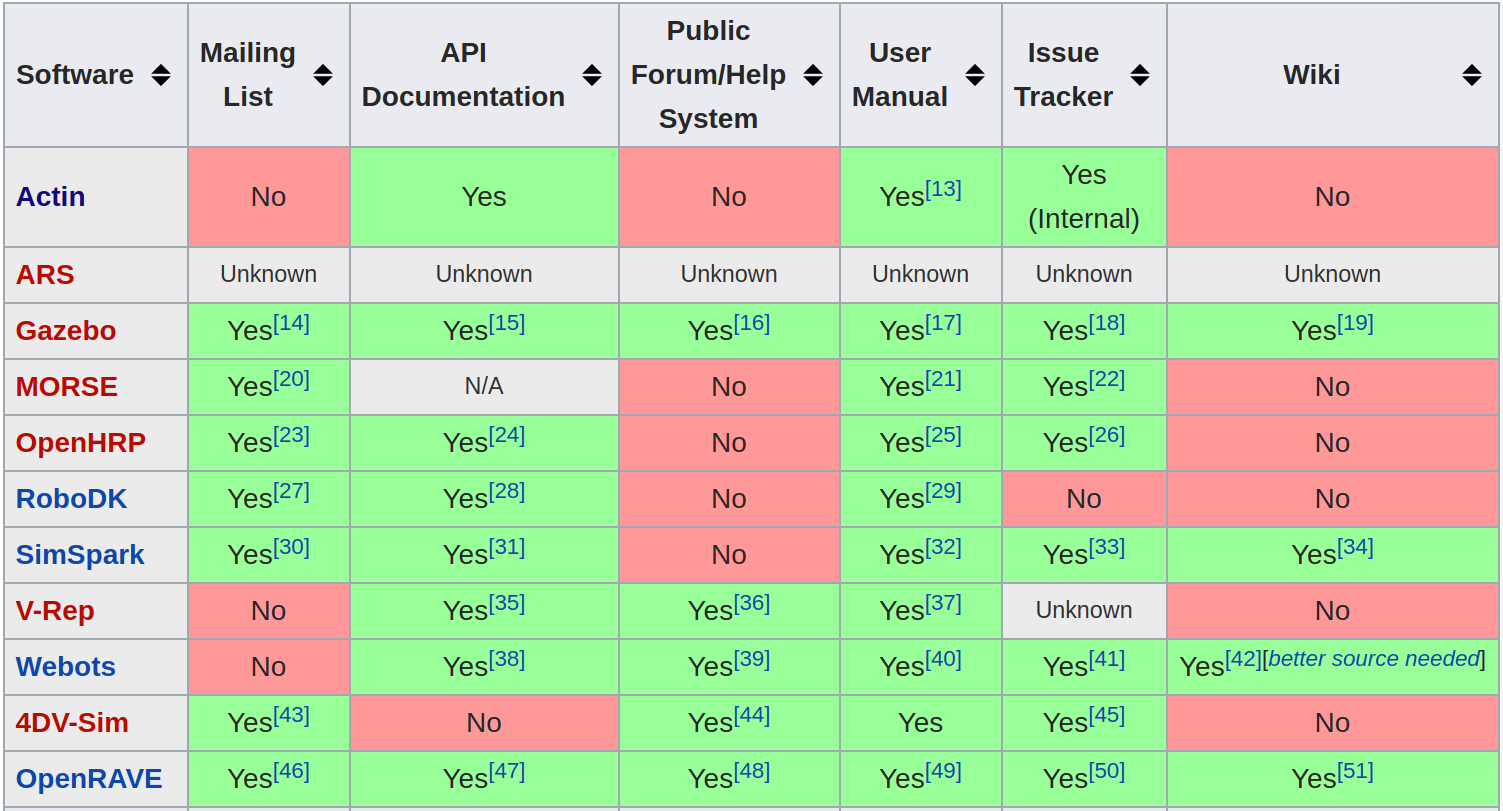
\includegraphics[width=.9\textwidth]{img/WikipTableRobSim.png}
  \caption{Types of support the different robot simulators provides. Taken from \href{https://en.wikipedia.org/wiki/Robotics_simulator}{\underline{Wikipedia}}(https://en.wikipedia.org/wiki/Robotics\_simulator)}
  \label{fig:infra}
\end{figure}

With Gazebo you can place a 3D model of the robot arm in a 3D scenario where you can place different other objects and for example test out different object avoidance algorithms. Gazebo comes with a good physics engine which give good simulation of the inertia and gravity impacting the robot. This is important because these are the two effects which impact the robot most. This will most likely make the transition between the simulated robot and the real robot less painful. \\

It can be useful to know that Gazebo is a simulation tool simulates the real world with physics. RVIZ is just a visualization tool used for visualize the inputs you are sending it and does not do any simulation. 




%For simulation and visualization in ROS, Rviz and Gazebo are used. Gazebo is a simulation environment with a good physics engine which can be used to simulate and test different control algorithms. Rviz is just a visualization tool to visualize the robot configuration and is great to use along with control of actual hardware. 



%\begin{figure}[htbp]
%  \centering
%  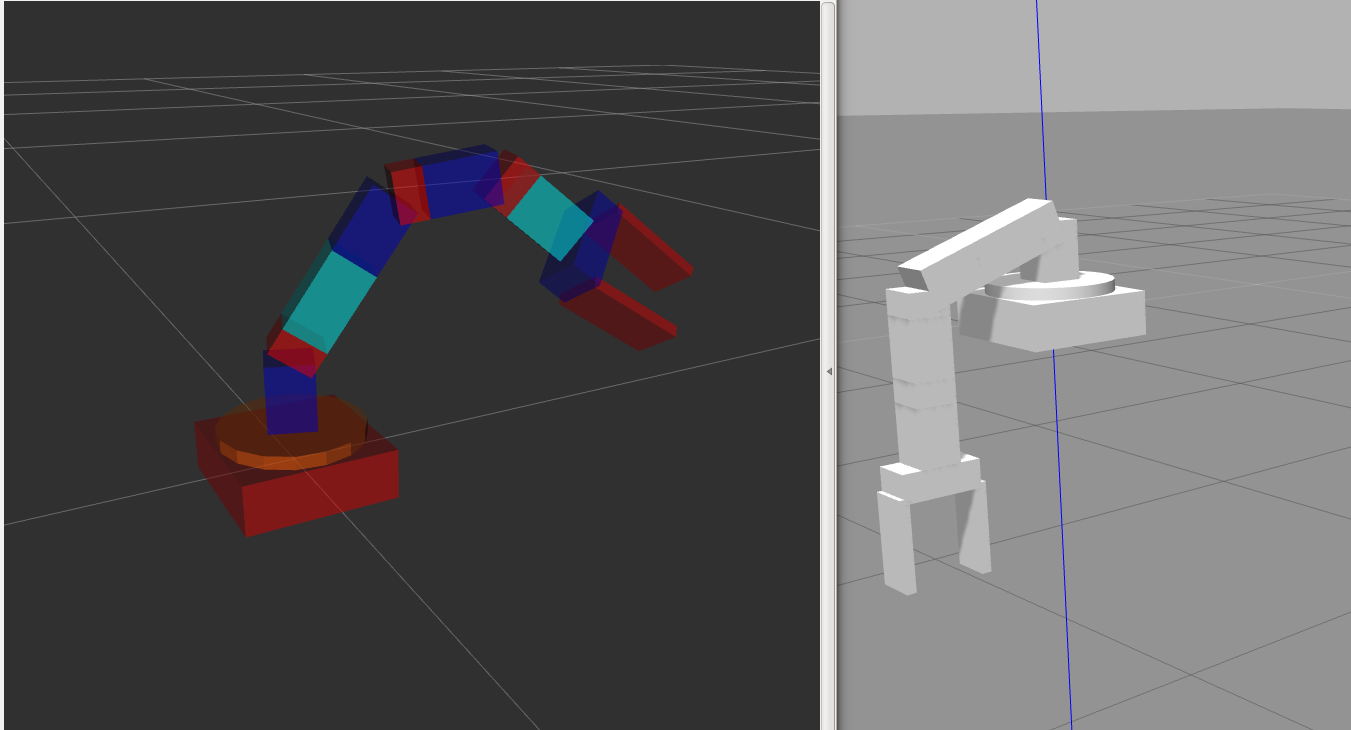
\includegraphics[width=.9\textwidth]{img/test.png}
%  \caption{Manipulators visualized in Rviz and Gazebo, respectively}
%  \label{fig:robot}
%\end{figure}


\section{File types}
All the code can be found at this Github repository: \href{https://github.com/Aarskog/robotarm}{\underline{rotbotarm}}\\

Now that the software to be used is found and installed the next step is to provide right tools to connect it together. Three different types of configuration files is therefore used and are listed below.
\begin{itemize}
    \item URDF - Describes the 3D model of the robot
    \item YAML - Describes the joint controllers and its parameters
    \item launch - Describes what processes to start on launch.
\end{itemize}
A more detailed description of the files is given in the sections below. 

\subsection{Unified Robot Description Format (URDF)}\label{sec:basicURDF}
The code used in the URDF is XML code which means that the syntax is very easy to understand. URDF consists of more, but there are two elements of the URDF that are important. The first is the link element that describes a part of the robot. In \lstref{lst:example} a link element is presented. This element describes a cylinder where the length and radius is given. 


\begin{lstlisting}[language=xml,caption={Base},label={lst:example}]
<link name="base_link">
    <visual>
        <geometry>
            <cylinder length="0.6" radius="0.2"/>
        </geometry>
    </visual>
</link>
\end{lstlisting}
The next important element is the joint element. When you have multiple links it is desirable to connect them together with joints. In \lstref{lst:jointexample} an example of a joint element is given. This gives the URDF parser information about how two links are connected. In this example \textit{link1} is the parent link of \textit{link2} the origin of the axes of rotation is given by the origin which is [0,0,1] which means that the origin of \textit{link2} is shifted 1 meter in the z direction relative to \textit{link2}. The joint type is revolute and it rotates about the z axis of the parent link. 

\begin{lstlisting}[language=xml,caption={Base},label={lst:jointexample}]
<joint name="joint_name" type="revolute">
    <parent link="link1"/>
    <child link="link2"/>
    <origin xyz="0 0 1"/>
    <axis xyz="0 0 1"/>
</joint>
\end{lstlisting}
This is the very basic for construction a object using URDF. A more detailed walkthrough is given when the method of construction of the robot is given in section \ref{sec:makingurdf}


\subsection{YAML-Yet Another Markup Language}
In the project, the joints.yaml file is the configuration file that states the torque con-troller for each joint. As per now a PID controller is used for each joint. This is basedon a SISO system for each joint. The dynamic equations of the manipulator is in fact acomplex nonlinear and multivariable system

\subsection{Launch files}
The launch files are used for starting up Gazebo,Rviz and the different nodes. It is also used to place the robot model into the simulation environment. The controller nodes are launched form control.launch.





\section{Description of the robot hand at hand}
In \figref{fig:robotAH} a picture of the actual robot is given. It is a five degrees of freedom robotic arm. Five degrees of freedom means in this case that the robot arm has five joints that we can control. In this case all the joints are rotational joints. 

\begin{figure}[htbp]
  \centering
  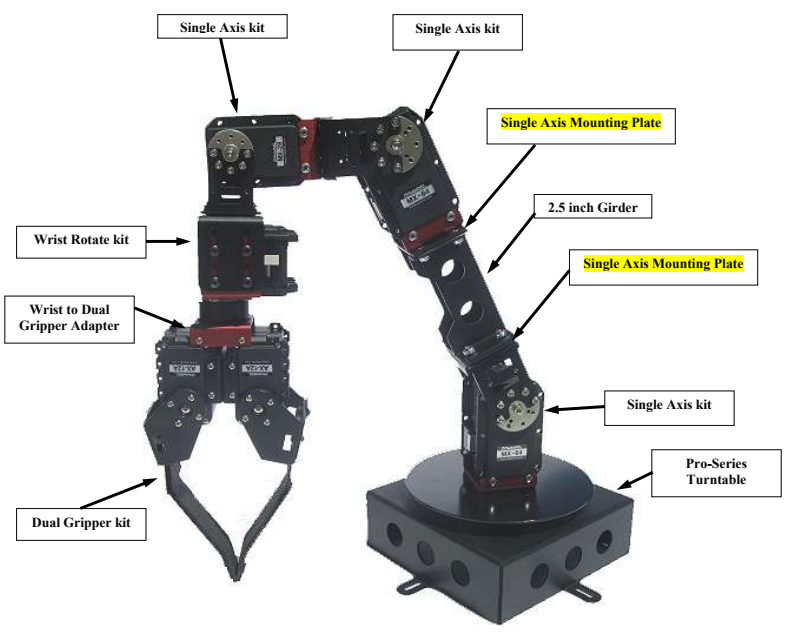
\includegraphics[width=.7\textwidth]{img/robotAH.png}
  \caption{Robot at hand}
  \label{fig:robotAH}
\end{figure}


\section{Making a visual model to be used in Gazebo}
The URDF includes mass and inertia as parameters which is possible to add a property of the joint. With this is mind the first to do is to find the mass of the different components that the robot at hand consists of. In \figref{fig:robotAH} for modelling and simulation the turntable base mass is not important to know since it is assumed that it is an unmoveable object that is stuck on the world frame. \\

\subsection{Dviding the robot into parts}
As briefly explained in section \ref{sec:basicURDF} the robot must be described as a series of links and joints. For the robot to be properly modelled with the URDF, it is desirable to find and classify the different parts of the robotic arm .  \\

In table \tabref{table:partlist} the different parts from the datasheet is listed. \tabref{table:partlist} is the initial list that was used as a base for constructing the robot. And in \figref{fig:utgangspunkt} the partnames are set their respective places on the robot. 

\begin{table}[htbp]
\centering
\caption{Partlist of the relevant parts taken from the datasheet and webpage of the robot}
\label{table:partlist}
    \begin{tabular}{ l r}
        \toprule
        Partname  & Amount \\
        \midrule
        MX-28T Pro-Series Turntable & 1\\
        MX-64T Pro-Series Single Axis kits& 2\\
        Pro-Series Single Axis Mounting Plates & 3\\
        2.5 inch(6.35cm) Pro Series Girder & 1 \\
        MX-28T Pro-Series Single Axis kit & 1 \\
        MX-28T Pro-Series Wrist Rotate kit & 1\\
        Pro-Series Wrist to Dual Gripper Adapter & 1\\
        Dual gripper kit with two AX-12A Servos& 1\\
               \bottomrule
    \end{tabular}
\end{table}



\begin{figure}[htbp]
  \centering
  \includesvg[width=.9\textwidth]{img/utgangpunktURDF.svg}
  \caption{Robot at hand}
  \label{fig:utgangspunkt}
\end{figure}



\subsection{Finding and guesstimating weights}
All the other weights above the turntable must be known. Unfortunately the datasheet does not give specific information about all of the parts. More of items were found in the webstore, but not all. The rest had to be guesstimated. For example the mass of circular plate which the rest of the arm stands on is not given explicitly. In \tabref{table:partmass} the different masses of the parts are presented. 
\begin{table}[htbp]
\centering
\caption{Mass of parts}
\label{table:partmass}
    \begin{tabular}{l c r}
        \toprule
        Part  &  Weight(kg) & Estimated\\
        \midrule
        MX-28T Pro-Series Turntable Plate& 0.05 & yes\\
        MX-64T Pro-Series Single Axis kits& 0.126 & no\\
        AX Short Bracket (SSB-Short) & 0.01 & yes\\
        2.5 inch(6.35cm) Pro Series Girder & 0.0227 & no\\
        MX-28T Pro-Series Single Axis kit & 0.072 & no \\
        MX-28T Pro-Series Wrist Rotate kit & 0.127 & no\\
        Pro-Series Wrist to Dual Gripper Adapter & 0.126 & yes\\
        Dual gripper kit with two AX-12A Servos& 0.01 & yes\\
        \bottomrule
    \end{tabular}
\end{table}


\subsection{Moments of inertia}
The next thing that was necessary to find, is the different moments of inertia of the robotarm. As seen from \figref{fig:robotAH} the different parts have different shapes and lengths so it can be a challenge to find the exact moments of inertia. A simplification is therefore needed. The simplifictaion that is used is to model them as boxes with uniform weight distribution. Although inertia is important to get a good model of the real robot, this simplifictation should not have a big impact of the error in the modelling. To calculate the moment of inertia the width,length and height of the part are needed. To simplify the naming of the different parts the following names seen in \figref{fig:naming} are used.\\


\begin{figure}[htbp]
  \centering
  \includesvg[width=.9\textwidth]{img/utgangpunktURDFWithNaming.svg}
  \caption{Naming}
  \label{fig:naming}
\end{figure}

\begin{table}[htbp]
\centering
\caption{Measurements of parts}
\label{table:measurements}
    \begin{tabular}{l c c c r}
        \toprule
        Part  &  x - Width(meter) & y - Length(meter) & z - Height(meter)\\
        \midrule
        Base & 0.1143 & 0.1143 & 0.0381\\
        Turntable & 0.055(radius) & NA & 0.01\\
        Motor2345 & 0.0356 & 0.0355 & 0.0506 \\
        Bracket123 & 0.0356 & 0.0355 & 0.0206 \\
        Girder & 0.0356 & 0.0355 & 0.0635\\
        Adapter & 0.0356 & 0.0710 & 0.0253\\
        Left/right finger & 0.03568 & 0.0089 & 0.08\\
        \bottomrule
    \end{tabular}
\end{table}


The complete documentation on the different parts is not complete this means that some of the lengths has to be guesstimated. In the simplified model (\figref{fig:naming}) there are only boxes except the turntable which is a small cylinder. For the boxes the following inertia matrix is used

\begin{align*}
    I = 
    \begin{bmatrix}
        I_{xx} & 0 & 0\\
        0 & I_{yy} & 0\\
        0 & 0 & I_{zz}
    \end{bmatrix}
\end{align*}
where
\begin{align*}
    I_{xx} &= \frac{1}{12}m(height^2+length^2)\\
    I_{yy} &= \frac{1}{12}m(height^2+width^2)\\
    I_{zz} &= \frac{1}{12}m(length^2+width^2)
\end{align*}
for the parts which are modelled as boxes and 
\begin{align*}
    I_{xx} &= \frac{1}{12}m(3r^2+height^2)\\
    I_{yy} &= \frac{1}{12}m(3r^2+height^2)\\
    I_{zz} &= \frac{1}{2}mr^2
\end{align*}
for the cylindrical turntable. 

\begin{table}[htbp]
\centering
\caption{List of inertias. Base is left out because it is fixed to the world frame and it is not neceassary to calculate this inertia}
\label{table:inertia}
    \begin{tabular}{l c c r}
        \toprule
        Part  &  $I_{xx}$ & $I_{yy}$ & $I_{zz}$\\
        \midrule
        Turntable & $3.82\cdot10^{-5}$ &  $3.82\cdot10^{-5}$ &$2.27\cdot10^{-4}$\\
        Motor2345 & $4.01\cdot10^{-5}$  & $4.01\cdot10^{-5}$  & $2.65\cdot10^{-5}$ \\
        Bracket123 & $1.40\cdot10^{-6} $ & $1.40\cdot10^{-6} $ & $2.10\cdot10^{-6} $ \\
        Girder & $1.00\cdot10^{-5} $ & $1.00\cdot10^{-5} $ & $4.80\cdot10^{-6} $\\
        Adapter & $5.97\cdot10^{-5} $ & $2.00\cdot10^{-5} $ & $6.62\cdot10^{-5} $\\
        Left/right finger & $~0$ & $~0$ & $~0$\\
        \bottomrule
    \end{tabular}
\end{table}

The moments of inertia are very small, and axis of rotation needs to be checked. It is also unknown how the URDF reader uses the inertias and how much it is up to the user to do adjustments. When construction the robot it is built in sequence from the bottom and up by adding part by part. The parent link of the first part is the world frame.

\subsection*{Constructing the robot}\label{sec:makingurdf}
Now everything need to make the URDF file is found and the calculations needed to be done is done. The first object to be made is the base. 

\begin{lstlisting}[language=xml,caption={Base}\label{lst:base}]
<link name="base_link">
    <visual>
        <geometry>
            <box size ="${basex} ${basey} ${basez}"/>
        </geometry>
        <origin xyz="0 0 0" rpy="0 0 0"/>
    </visual>
    <inertial>
        <origin xyz="0 0 0" rpy="0 0 0"/>
        <mass value="2"/>
        <inertia ixx="1" ixy="0" ixz="0" iyy="1" iyz="0" izz="1" />
    </inertial>
    <collision>
        <origin xyz ="0 0 0"/>
        <geometry>
            <box size ="${basex} ${basey} ${basez}"/>
        </geometry>
    </collision>
</link>
\end{lstlisting}

In \lstref{lst:base} the XML based URDF code is presented. The declaration can be divided into three topics: Visual, inertal and collision. The different topics are self explanatory. The valuses chosen for the values chosen for the moment of inertia and the mass is chosen arbitrary since the based is fixed to the world and is not supposed to move. Then the turntable is modelled in the same way. Now that two links has been made in the model a joint object is needed.

\begin{lstlisting}[language=xml,caption={joint between base and turntable},label={lst:jointBTT}]
<joint name="base_to_turntable" type="continuous">
  <parent link="base_link"/>
  <child link="turntable"/>
  <origin xyz="0 ${0} ${(basez+turntable_height)/2}"/>
  <axis xyz ="0 0 1"/>
</joint>
\end{lstlisting}
 Above in \lstref{lst:jointBTT} the joint object is given. Again it is pretty much self explanatory. The biggest challenge here is to place the turntable at the right position relative to the base and get it to rotate the way it is supposed to rotate. When placing the origin of the joint it is adjusted relavtive of the origin of the parent link. Moving the joint origin will move the origin of the child link. Therefore the join origin is set to half of the sum of the height of the two links. This will place the turntable on top of the base. The axis is the axis of rotation which is the z-axis. This was the joint for the twisting joint. The other twisting joint is modelled the same way. For the rotational joints(joint 2,3 and 4) the axis of rotation is about the x-axis relative to the its parent link. \\
 
After all the links and joints are placed the model needs to be spawned in Gazebo. To do this a launch file is used. To start Gazebo with an empty world the following code shown in \lstref{lst:empty} is used
\begin{lstlisting}[language=xml,caption={Start Gazebo with empty world},label={lst:empty}]
<include file="$(find gazebo_ros)$/launch/empty_world.launch">
  <arg name="paused" value="false"/>
  <arg name="use_sim_time" value="true"/>
  <arg name="gui" value="true"/>
  <arg name="headless" value="false"/>
  <arg name="debug" value="false"/>
</include>
\end{lstlisting}
the last two elements are given in \lstref{lst:l2} where the first line is a script that needs to be ran since macroes is used. The second line creates the node that will spawn the robot into Gazebo. 
\begin{lstlisting}[caption={Spawn robot model in Gazebo},label={lst:l2},language=xml]
  <param name="robot_description" command="$(find xacro)/xacro.py $(arg model)" />

  <node name="urdf_spawner" pkg="gazebo_ros" type="spawn_model"
        args="-z 0.01905 -pause -urdf -model robot -param robot_description" respawn="false" output="screen" />
\end{lstlisting}